\section{Descrizione del modello}

\subsection{Overview}
\begin{frame}{Approccio ad agenti}
	\begin{itemize}
		\item \textbf{Sistema multiagente} sviluppato in Python con il framework Mesa
		\begin{itemize}
			\item \textbf{Ambiente}: supermercato
			\begin{itemize}
				\item Il supermercato è una struttura divisa in zone, composta da code e casse
				\item I clienti entrano nel supermercato per fare la spesa minimizzando il tempo impiegato
			\end{itemize}
			\item \textbf{Agenti}: clienti e casse
		\end{itemize}
		
		\item I clienti sono agenti intelligenti (pianificano e decidono) con una componente impredicibile che fa emergere un comportamento complesso interagendo con gli altri agenti
	\end{itemize}
\end{frame}

\begin{frame}{Ambiente}
	
	\begin{figure}[H]
		\centering
		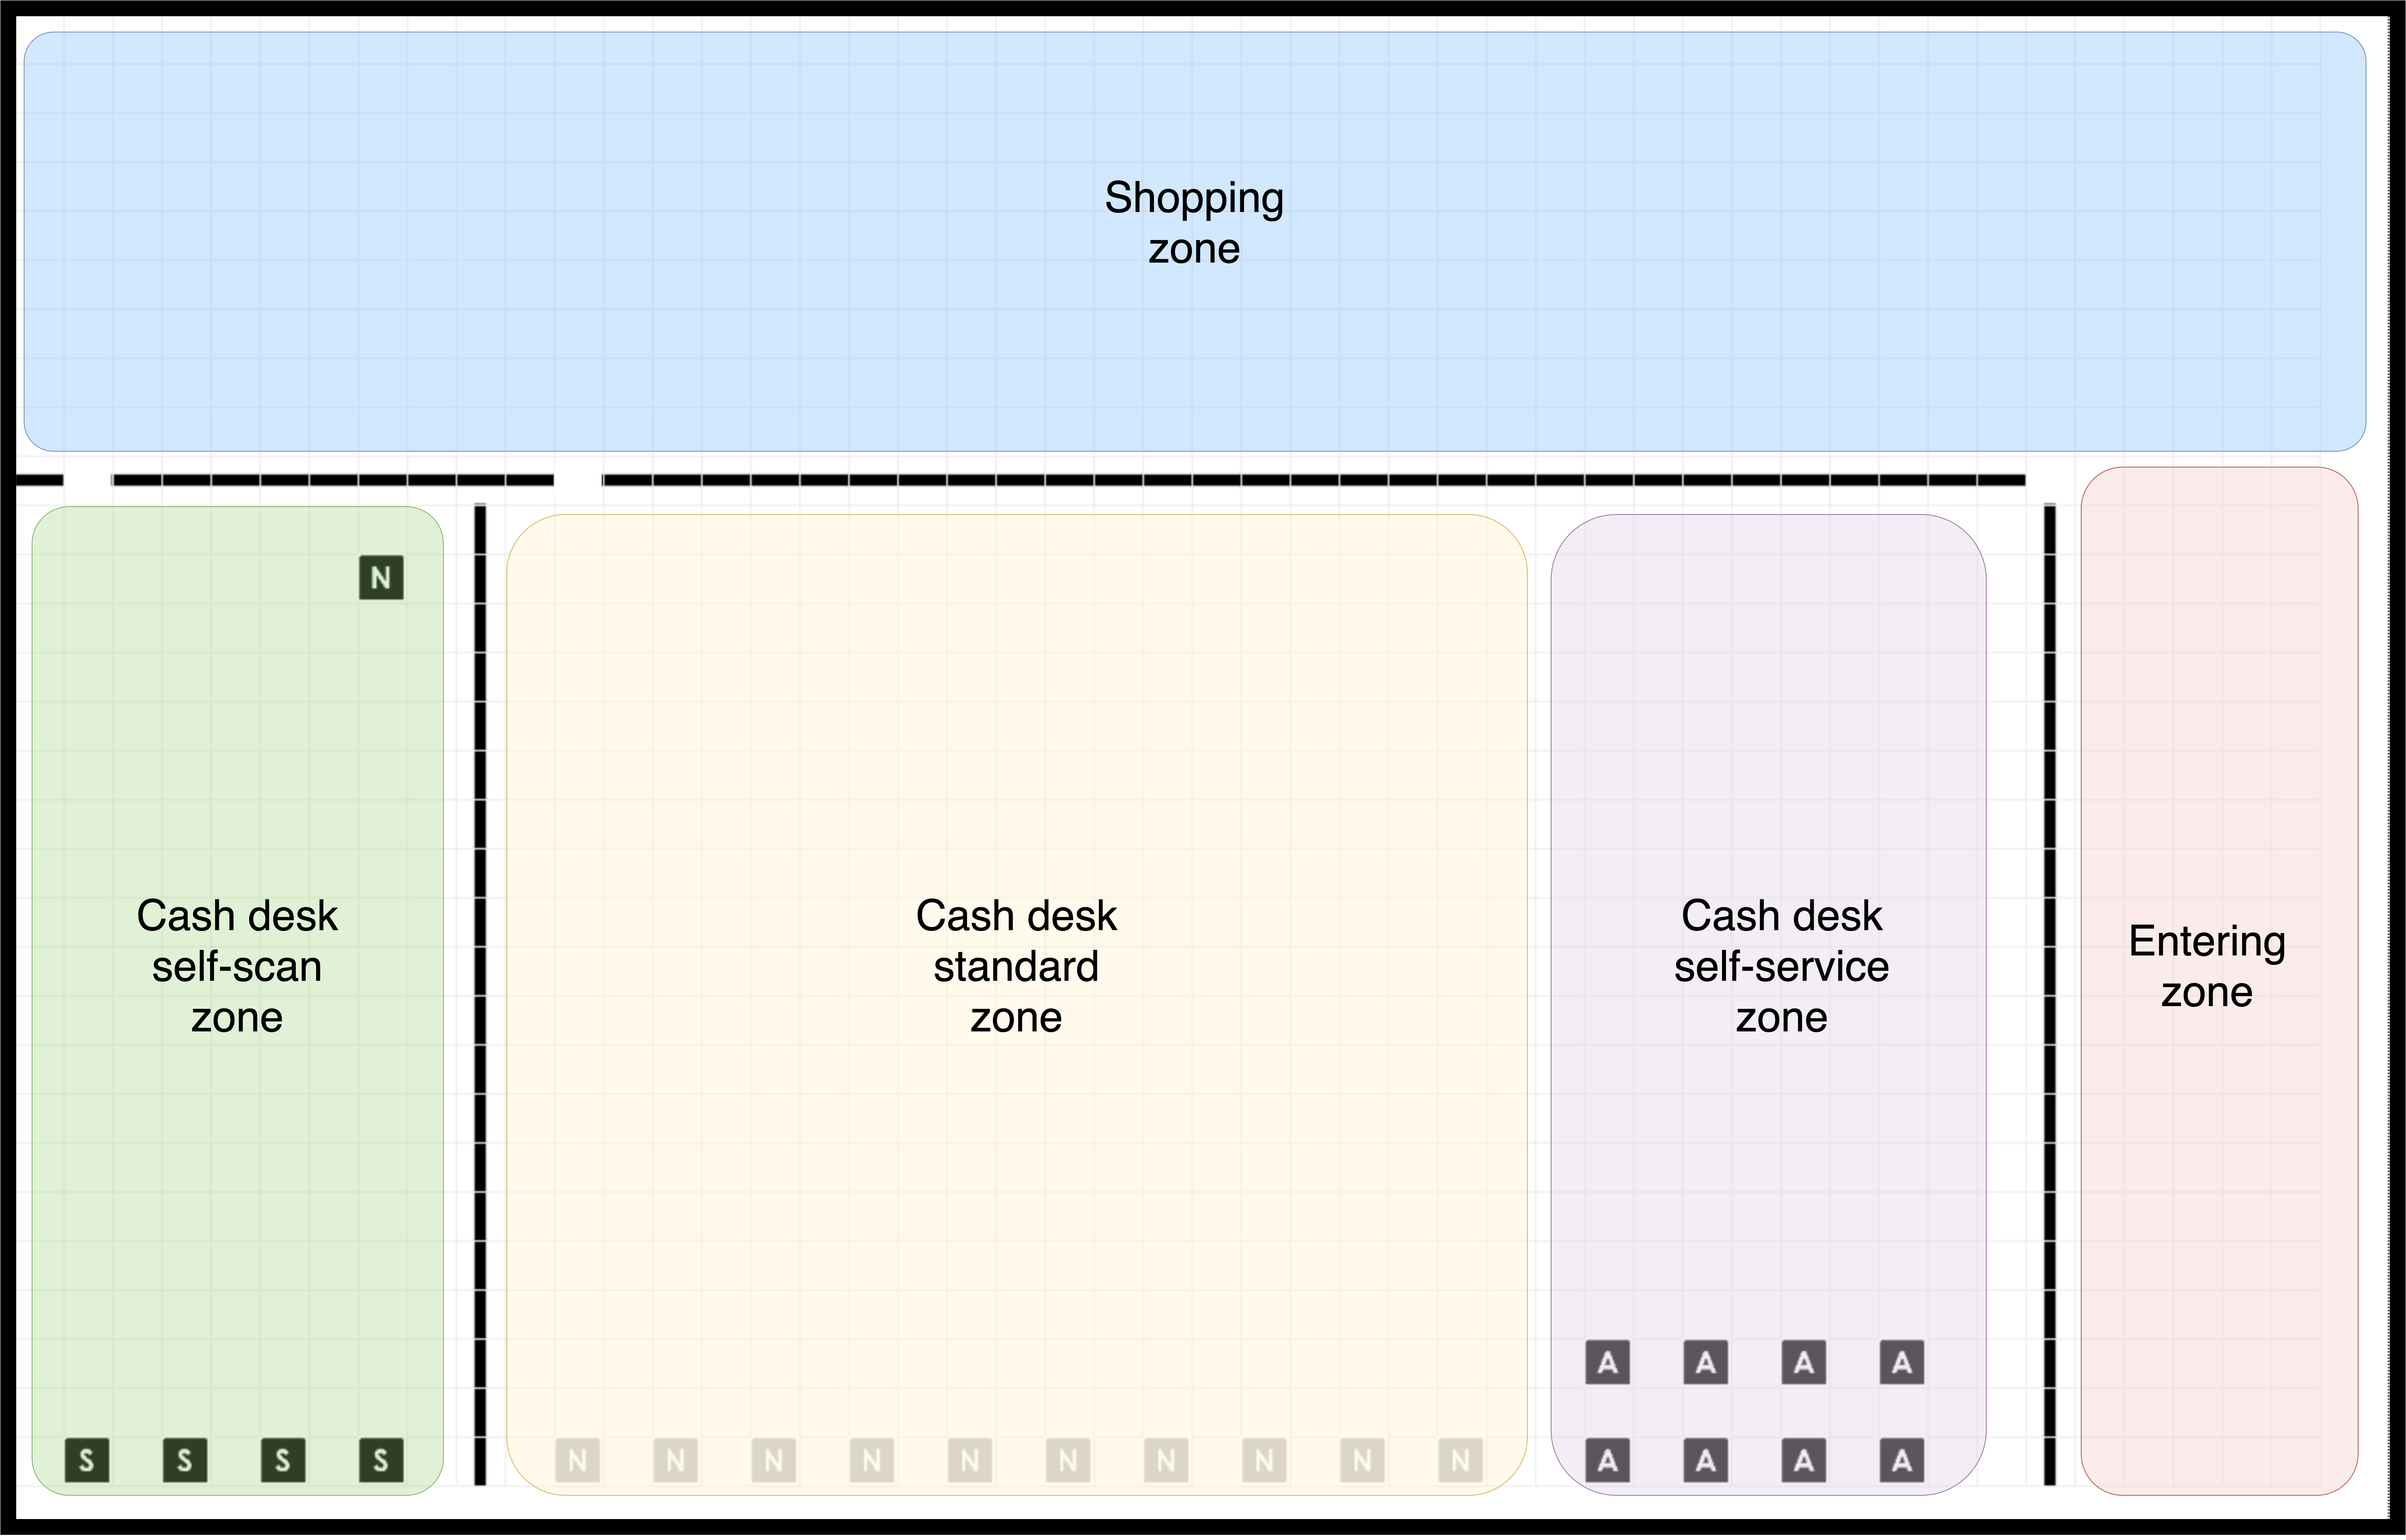
\includegraphics[width=9cm]{"../report/images/supermarket-start-zones.png"}
		\caption{Stuttura del supermercato diviso in zone.}
		\label{fig:supermarket_zones}
	\end{figure}
	
	
\end{frame}


\begin{frame}{Ambiente}
	\begin{figure}[H]
		\centering
		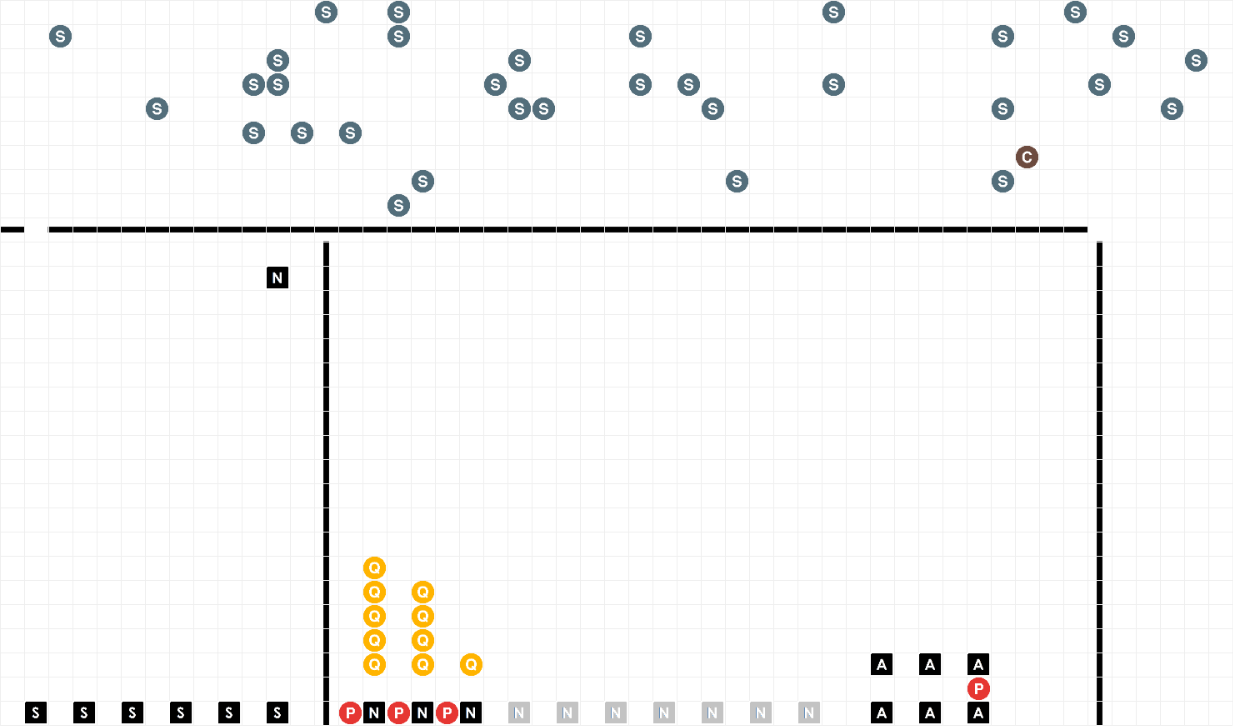
\includegraphics[width=9cm]{"../report/images/supermarket-execution.png"}
		\caption{Interazione tra agenti e ambiente.}
		\label{fig:supermarket_execution}
	\end{figure}	
\end{frame}

%----------------------------------------------------------------------------------------

\subsection{Agenti del modello}

\begin{frame}{Agente Cliente}
	\begin{itemize}
		\item I clienti sono gli agenti principali, si muovono nel supermercato con l'obiettivo di fare la spesa e attendere il minimo tempo possibile in coda
		\item Per minimizzare il tempo in coda il cliente usa strategie di \textbf{scelta della coda} e di \textbf{jockeying}, quindi ha bisogno di una pianificazione
		\item Il cliente è un agente di tipo \textit{utility-based} perchè per la pianificazione e la valutazione dei tempi d'attesa utilizza una utility function
	\end{itemize}
\end{frame}

\begin{frame}{Agente Cliente - workflow}
	\begin{enumerate}
		\item \textbf{Attesa all'entrata del supermercato}: l'agente è in attesa fino a che non può mettersi nella zona d'entrata.
		\item \textbf{Fase di shopping}: si muove nella zona di shopping e inizia a raccogliere elementi fino a raggiungere il \textit{basket size} desiderato; questa fase dipende dalla velocità di shopping, un parametro del modello.
		\item \textbf{Scelta della coda}: finita la spesa, deve scegliere la cassa in base alla utility function; viene scelta la coda $q^*$ tale che
		\[q^* = \operatorname*{argmin}_{q \in Q} f(q)\]
		dove $Q$ è l'insieme delle code dedicate e $f$ varia con la strategia.
	\end{enumerate}
\end{frame}
\begin{frame}{Agente Cliente - workflow}
	\begin{enumerate}
		\item \textbf{Attesa in coda e jockeying}: mentre il cliente è in coda può decidere di lasciarla per una coda migliore. Considera le 2 code adiacenti (parametro del modello) alla propria e per ognuna calcola la coda migliore secondo la sua strategia di jockeying. Se il "guadagno" risulta maggiore di un certo \textbf{threshold}, allora il cliente può decidere di cambiare coda. Si estrae quindi un numero casuale che determina se cambiare coda o no (perchè non tutte le persone fanno jockeying).
		\item \textbf{Attesa alla cassa}: il cliente viene servito dalla cassa e deve attendere la fine del pagamento per uscire dal supermercato.
	\end{enumerate}
\end{frame}


%----------------------------------------------------------------------------------------


\begin{frame}{Agente Cassa}
	\begin{itemize}
		\item I clienti, una volta conclusa la fase si di spesa, scelgono una coda in attesa di essere serviti in cassa per il pagamento.
		\item Ogni cassa ha al più una coda associata.
		\item La cassa è un'agente di tipo \textit{model-based reflex}, in cui lo stato è il cliente che si sta processando in un determinato momento.
		\item Il comportamento di una cassa è piuttosto semplice:
		\begin{enumerate}
			\item Prendi un cliente dalla coda (se disponibile)
			\item Processa il cliente
			\item Ripeti
		\end{enumerate}
		\item Le code (FIFO) ammissibili per ogni cassa sono di 2 tipi:
		\begin{enumerate}
			\item Coda dedicata: ogni cassa ha una coda dedicata
			\item Coda condivisa: una coda è associata a più casse, tutte le casse serviranno i clienti che si sono accodati alla coda condivisa
		\end{enumerate}
		\item Nel modello sono state modellate 4 tipi di casse diverse.
		
	\end{itemize}
\end{frame}

\begin{frame}{Agente Cassa - Tipo 1: Standard}
	\begin{itemize}
		\item Rappresenta la classica cassa di un supermercato.
		\item Questa cassa può avere una coda dedicata o condivisa, in entrambi i casi:
		\begin{enumerate}
			\item Il cliente si accoda
			\item La cassa prende il primo cliente dalla coda
			\item Il cassiere processa gradualmente tutti gli articoli del cliente
			\item Ripeti
		\end{enumerate}		
	\end{itemize}
\end{frame}

\begin{frame}{Agente Cassa - Tipo 2: Self-service}
	
	\begin{itemize}
		\item Cassa in cui non è presente un cassiere ma è il cliente stesso a dover passare uno alla volta gli articoli acquistati.
		\item Tutte le casse self-service hanno una coda condivisa
		\begin{enumerate}
			\item Il cliente si accoda alla coda condivisa
			\item La cassa prende il primo cliente dalla coda
			\item Il cliente processa ogni articolo
			\item Il cliente lascia il supermercato
		\end{enumerate}		
	\end{itemize}
\end{frame}

\begin{frame}{Agente Cassa - Tipo 3: Self-scan}
	
	\begin{itemize}
		\item Il cliente scannerizza gli articoli durante la spesa mediante un dispositivo fornito dal supermercato.
		\item Avendo già scanerizzato gli articoli a priori non è necessario farlo in cassa.
		\item Vengono effettuati controlli a campione per verificare il corretto comportamento dei clienti (tutti gli articoli devono essere stati effettivamente scannerizzati durante la spesa).
		\item Tutte le casse hanno una coda condivisa
		\begin{enumerate}
			\item Il cliente si accoda alla coda condivisa
			\item La cassa prende il primo cliente dalla coda
			\item Nel caso in cui il cliente è stato estratto per una rilettura della spesa si reca ad una cassa riservata, altrimenti paga ed esce dal supermercato
		\end{enumerate}		
	\end{itemize}
\end{frame}

\begin{frame}{Agente Cassa - Tipo 4: Riservata}
	
	\begin{itemize}
		\item Comportamento analogo alla cassa standard.
		\item Ha una coda dedicata.
		\item Nel caso di rilettura alla cassa "self-scan", il cliente viene normalmente processato in questa nuova cassa.
		\item La rilettura può essere \textbf{parziale} (vengono controllati solo 10 elementi), o \textbf{totale} (viene controllata tutta la spesa).
		\item Nessun cliente può venire processato nella cassa riservata a meno di una rilettura.
	\end{itemize}
\end{frame}


%----------------------------------------------------------------------------------------


\begin{frame}{Considerazioni}
  \begin{itemize}
  \item Il modello da noi descritto é stato implementato con
    l'obbiettivo di essere facile da modificare.
    
  \item Il comportamento degli agenti viene gestito con una
    macchina a stati finita implementata tramite il pattern
    \textbf{State}.  Questo isola logicamente aspetti quali
    azioni da compiere e rappresentazione grafica da assumere in
    determinati stati.

  \item Dove esistono diversi approcci ad una scelta, per
    esempio nella scelta della coda, questi vengono gestiti con
    il pattern \textbf{Strategy}, dando possibilitá di scelta
    tra piú opzioni e una facilitazione nel crearne di nuove.

  \item I parametri che regolano il modello descritti a seguire
    sono configurabili a piacere.
  \end{itemize}
\end{frame}


%----------------------------------------------------------------------------------------


\begin{frame}{Parametri}
	\begin{itemize}
		\item Configurazione del supermercato:
		\begin{itemize}
			\item Dimensione delle zone (entering zone, shopping zone)
			\item Numero di casse (standard, self-service o self-scan + 1 riservata)
			\item Code N-fork o parallele per le casse standard
		\end{itemize}
		\item Parametro per l'errore di stima del basket size: usato nelle strategie di scelta della coda e jockeying per simulare l'errore commesso dagli umani nello stimare la quantità di oggetti nei carrelli
		\item Jockeying:
		\begin{itemize}
			\item Numero di code adiacenti considerate
			\item Threshold
			\item Probabilità di fare jockeying
		\end{itemize}
		\item Distribuzione dei clienti in entrata (presa dai dati di Antczak e altri\footnotemark)
		\item Distribuzione dei basket size (presa dai dati di Antczak e altri\footnotemark[\value{footnote}])
		\footnotetext{Antczak, Tomasz and Weron, Rafał and Zabawa, Jacek, 2020}
	\end{itemize}
\end{frame}

\begin{frame}{Parametri - distribuzione dei clienti}
	Nella figura si riporta la distribuzione di entrata dei clienti reale e la distribuzione generata effettuando normalizzazione, media e divisione per step.
	\begin{figure}[H]
		\centering
		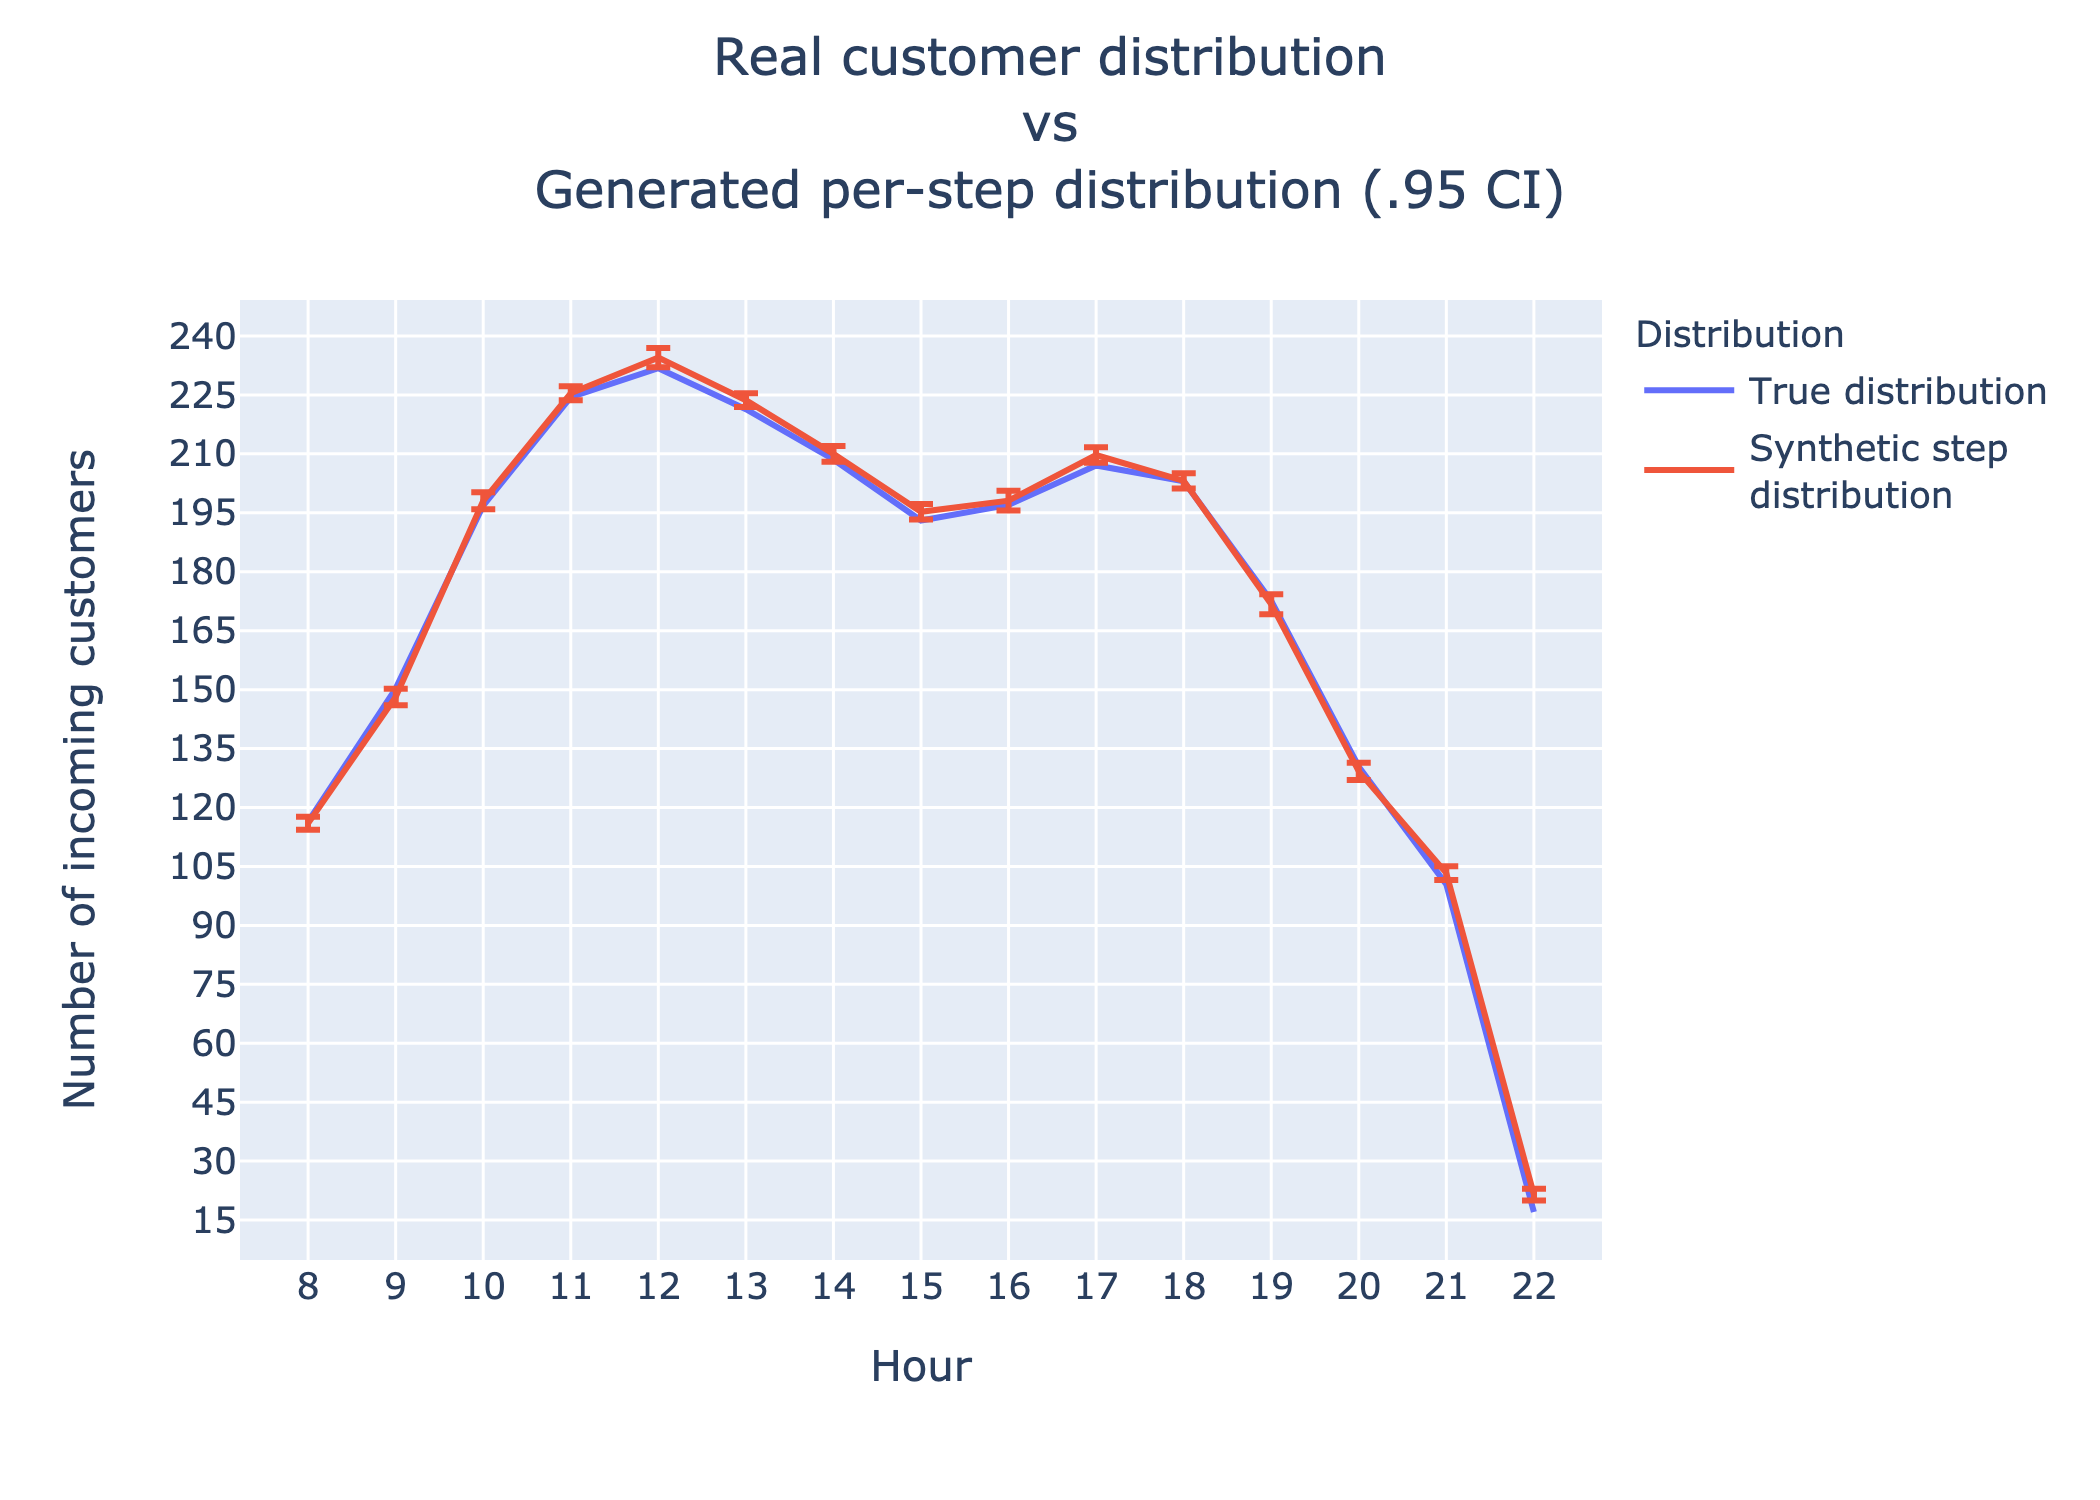
\includegraphics[width=9cm]{"../report/images/real_vs_synthetic_distribution.png"}
		\label{fig:dist_basket_size}
	\end{figure}
\end{frame}

\begin{frame}{Parametri - distribuzione dei basket size}
	Nella figura viene mostrata la distribuzione reale dei dati e la distribuzione esponenziale derivata aggregandoli, la quale viene usata nel modello per generare il basket size di ogni cliente.
	\begin{figure}[H]
		\centering
		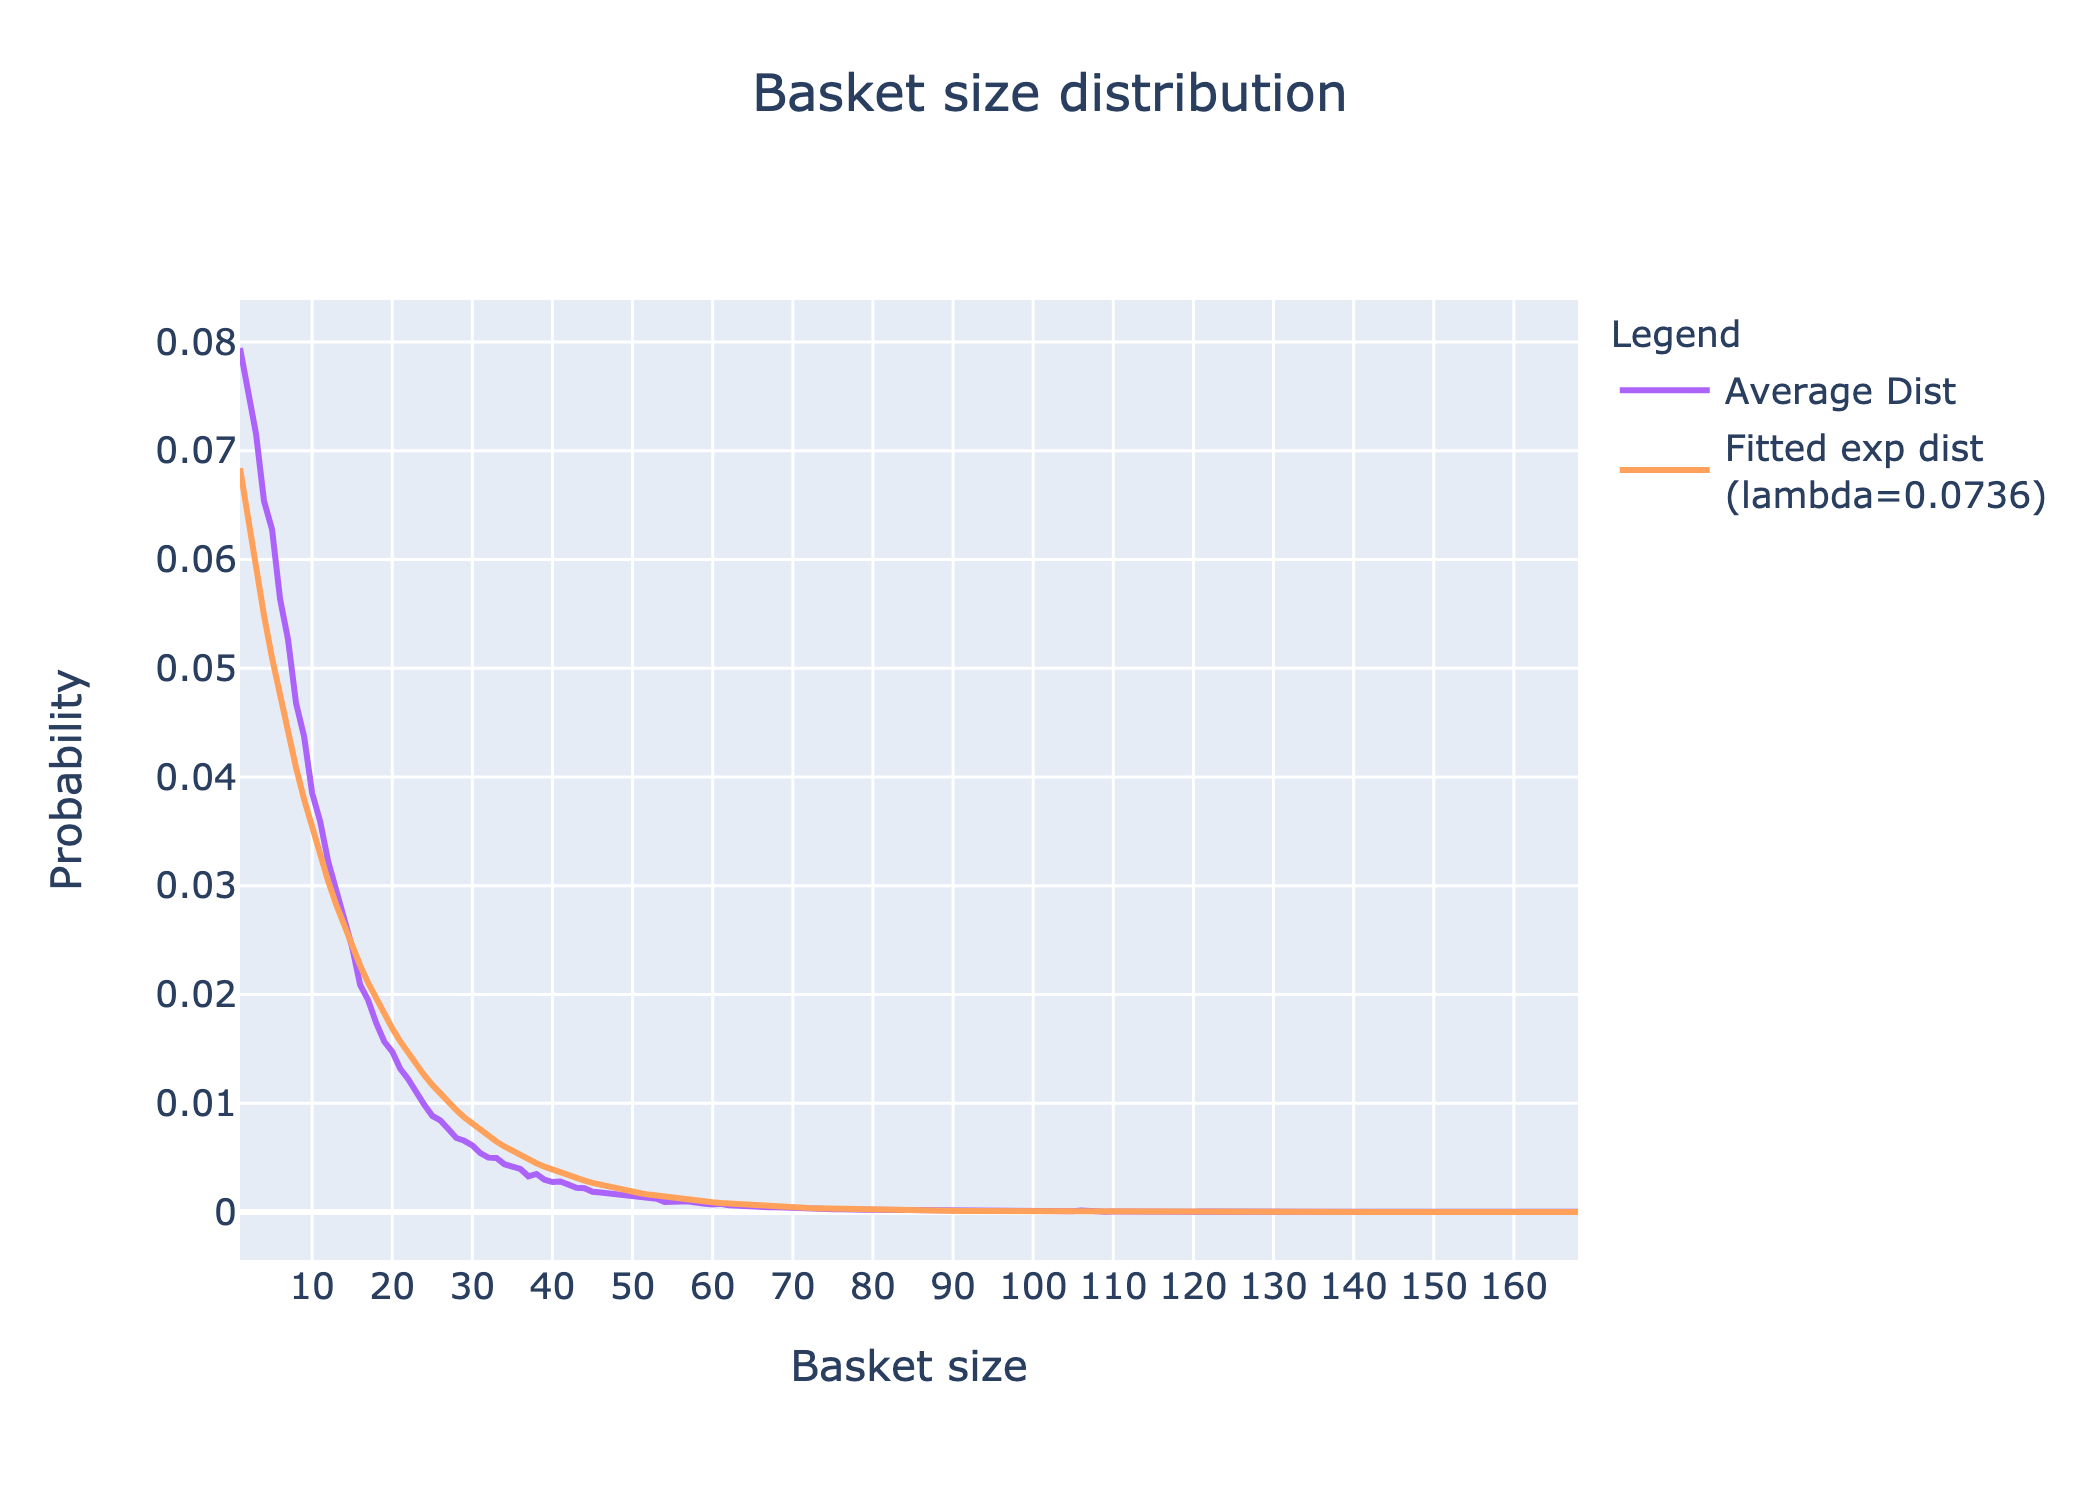
\includegraphics[width=9cm]{"../report/images/basket_size_fitted.png"}
		\label{fig:dist_basket_size}
	\end{figure}
\end{frame}

\begin{frame}{Parametri}
	\begin{itemize}
		\item Parametri di tempo:
		\begin{itemize}
			\item Durata di uno step (attualmente 30 secondi)
			\item Velocità di shopping del cliente: numero di articoli messi nel carrello ad ogni step
			\item Tempo di elaborazione della spesa da parte delle casse: per le self-scan è 1 step, per le standard e le self-service è governato dai parametri $a, b, \alpha, \beta \in \mathbb{R}$, presi dall'articolo di Antczak e altri sopra citato.
		\end{itemize}
	\end{itemize}
\end{frame}